\section{The Problem of Unintended Reuse}

Unintended reuse is a serious and fundamental problem in the
interpretation of images. We can consider an interpretation of an
image to consist of various assertions about the contents of the
image. We can characterize these assertions by asking what region of
the image they refer to, and in particular how large that region is.

Compositional models are those models in which the quality or
plausibility of a high-level assertion (i.e., one that refers to a
large image region) is defined recursively in terms of the quality of
lower-level assertions (in a way amenable to dynamic programming). It
is thus a general problem of compositional models that we can only
efficiently and exactly compute the quality of high-level assertions
by allowing them to depend on low-level assertions that are
contradictory. This can then result in incoherent interpretations of
the image. In our case, straight-forward maximization of the
likelihood under the statistical model described above yields curves
that have many self intersections; curves in whcih long contours are
used multiple times, often in opposite directions; and curves which do
not enclose any area.

In general, we cannot sacrifice efficiency beyond a certain point, and
so we must search for a coherent interpretation which may not score
the highest, even among coherent interpretations.

One approach to solving this problem, used in \cite{jin-geman},
is to fix various low-level assertions that seem likely, and eliminate
incompatible low-level assertions from consideration.
\marginnote{Discuss more?} In our case, this approach does not yield
good results. 

There is another body of research in computer vision that uses Markov
random fields in order to select a set of compatible low-level
assertions. These methods are quite robust to noise when used
correctly. We adapt these methods to our present need as follows:
rather than defining a statistical model over the low-level assertions
used in our shape model, we define a statistical model over related
low-level assertions that resolve certain fundamental ambiguities in
our global model. We call this model a local interpretation model. Our
goal in selecting a local interpretation is not to interpret the
image, but rather to eliminate problematic sources of incoherence in
our global interpretations. Since our global model suffered greatly
from the problem of reusing a long contour in opposite directions, a
fundamental component of our local interpretation model is assigning
orientations locally to edge pixels. If these edge pixels participate
in the final global interpretation, the local orientation constrains
them to be used only in one direction, preventing the previously
mentioned strategy of forming incoherent parse trees. If the edge
pixels do not participate in the final global interpretation, the
orientation assigned to them does not mean anything.

Our approach is motivated by the following observation: when we reuse
a line segment, we tend to reuse it in opposite directions. This is
especially true if the curve is the boundary of an object. Using the
line segment twice in the same direction would make it impossible to
assign a consistent inside and outside to the pixels of the image.

In problematic parses, we tend to see a segment used once forward and
once backward, or to see it used twice forward and once backward.

Thus, if we knew the ``correct'' orientation of the line, we would
know that only one of these directions is legitimate, and we could
penalize the other orientation.

Similarly, if we knew which pixels were inside the curve, and which
were outside, parsing would be easy.

We claim that we can, with some luck, use Gibbs sampling and/or
simulated annealing to discover the correct orientations and the
correct interior.

\section{Local Interpretations}

We wish to search over local interpretations. A local interpretation
is a function $L: P \to D \cup Z$, \marginnote{Add disjoint union
  symbol} where $P$ is the set of pixels, $D$ is a set of directions,
and $Z$ is a set of region labels. In the simplest case, $Z$ will be
$\{0,1\}$, with $1$ being the label assigned to pixels inside the main
shape, and $0$ being the label assigned to pixels outside the main
shape. We will assign a probability to each local interpretation, and
do approximate inference to select a likely one. The probability of
$L$ will be defined as
$$ \prod_{p\in P} \phi_p(L), $$
where
$$ \phi_p(L) = \begin{cases} \epsilon_p(L) \omega_p(L) & L(p)\in D\\ (1-\epsilon_p(L)) \sigma_p(L) & L(p)\in Z\end{cases}.$$
% $$\phi_p(L) = \frac{e^{z_p(L)/T}}{e^{z_p(L)/T} + e^{-z_p(L)/T}},$$
% and 
% $$z_p(L) = x_p(L) + \sum_{q} y_{p,q}(L).$$

% Here $x_p(L)$ measures the desire of $p$ to be an edge pixel, and the
% consistency of its assigned orientation with our previous global
% parse. $y_{p,q}(L)$ measures the consistency of orientations,
% consistency of region labels, and models interactions between
% orientation assignment and region labels.

Finding a local interpetation is a combination of three problems:
\begin{itemize}
\item Edge detection: if $L(p)\in D$, then $p$ is an edge pixel. If
  $L(p)\in Z$, then $p$ is a non-edge pixel. We model this using the
  distribution $\epsilon_p(L)$.

\item Segmentation: $\{ L^{-1}(z)\mid z\in Z\}$ is a coarse
  segmentation of the non-edge pixels in the image. We model this
  using the distribution $\sigma_p(L)$. Since we will generally be
  using $Z=\{0,1\}$, this can also be thought of as splitting the
  image into figure and ground.

\item An assignment of orientations to edges, modeled by the
  distribution $\omega_p(L)$. This is not a standard problem in
  computer vision, and thus deserves more explanation. Orientation
  assignment can be thought of as a low-level or early vision
  equivalent of contour grouping. Many contour groupings will be
  compatible with a given orientation assignment, but a ``good''
  orientation assignment will allow most reasonable contour groupings
  and disallow most unreasonable contour groupings.  \marginnote{Talk
    about contour grouping, and explain what makes a contour grouping
    good?}

\end{itemize}

By considering the three problems simultaneously, we hope to be able
to use information from a candidate solution to one problem to guide
our choice of solution in the other problems.

Note that the probability can be factored over the three problems,
which has been our approach during inference.

We perform the optimization using Gibbs sampling. In order to push the
local interpretation towards optimal hypotheses, we perform simulated
annealing, where the proposal distribution depends on a temperature
parameter $T$, with lower $T$ corresponding to more peaked
distributions. We start with high $T$ and gradually decrease $T$,
performing Gibbs sampling at temperatures $T_k > T_{k-1} > \cdots >
T_1$. This is known as a cooling schedule, and is a standard
technique.\marginnote{Get desc. of Gibbs sampling from Bishop or Geman
  and Geman}

\marginnote{How do we initialize?}

Let $\vec{g}(p) = (I_x(p), I_y(p))$ be the gradient of the image
intensity at pixel $p$. We define the rotated gradient $\vec{r}(p) =
(I_y(p), -I_x(p))$.


\subsection{Edge Model}

We are currently using a non-probabilistic model for $\epsilon$. We
simply use the output of the Canny edge detector \cite{canny}. In the
future we hope to experiment with a probabilistic model here,
especially one that can make use of the context provided by the other
two parts of the local interpretation model to improve the accuracy of
the edge map.

\subsection{Segmentation}

Let us assume that $Z=\{0,1\}$, so that we are splitting non-edge
pixels into those we believe to be inside the curve, and those we
believe to be outside the curve. We would like this division to meet
the following criteria:
\begin{itemize}
\item Adjacent non-edge pixels should agree on whether they are in the
  interior.

\item If pixel $p$ is in the interior, then the orientation at a
  nearby edge pixel $q$ should be going clockwise, i.e., the angle
  between $q-p$ and the orientation at $q$ should be less than 180
  degrees. If we are in the exterior, they should be going
  counter-clockwise. We capture this notion by considering a modified
  version of the cross product:
$$(x_1,y_1) \times (x_2,y_2) = x_1 y_2 - x_2 y_1.$$
By comparing this with the traditional cross product on vectors with
no $z$ component
$$(x_1,y_1,0) \times (x_2,y_2,0) = (0,0,x_1 y_2 - x_2 y_1),$$
we can see that $$v_1 \times v_2 = ||v_1|| ||v_2|| \sin \theta,$$
where $\theta$ is the angle between $v_1$ and $v_2$.
\end{itemize}

Let $i_p(L) \in \{-1,0,1\}$, with $i_p(L)=1$ when $p$ is an interior
pixel, $i_p(L) = -1$ when $p$ is an exterior pixel, and $i_p(L)=0$
when $p$ is an edge pixel. We can then enforce our critera using the
following $\sigma_p$:
\begin{align*}
\sigma_p(L) &= \frac{e^{x_p(L)/T}}{e^{x_p(L)/T} + e^{-x_p(L)/T}},
\intertext{where}
x_p(L) &= \beta C(p) + \sum_{q\sim p} i_q(L)\\
\intertext{and}
C(p) &= \sum_{q: L(q)\in D} e^{-||q-p||^2/\gamma^2} \left( O(q) \vec{r}(q) \right) \times \left( \frac{(q-p)}{||q-p||} \right).\\
\end{align*}

For efficiency, we can limit the sum over $q$ to those $q$ where
$e^{-||q-p||^2/\gamma^2}$ is non-trivial.

\subsection{Orientation Assignment}

The ideal orientation assignment will trace out object boundaries
clockwise, and will have no sources or sinks, except at T-junctions
and the beginning and end of internal edges, where it will have a
source or sink according to specific rules:

\begin{itemize}
\item T-junctions: in the neighborhood of the T-junction, there should be
one differentiable curve that goes through the neighborhood and the
junction point, and one differentiable curve that ends at the junction
point, possibly at a right angle.

\item Internal edge caps: there should be a differentiable curve that begins
or ends at the point. Internal edge cap always indicate self-occlusion.

\item There are other more exotic junctions, like X-junctions and
Necker-cube junctions, but they are probably not common enough to care
about for our inference problem. (This is one advantage to considering
the local version of the problem.)
\end{itemize}

The connection to contour grouping is as follows: if two adjacent edge
pixels are assigned dissimilar orientations, then it is unlikely that
they are part of the same contour, and we will say that the
orientation assignment is incompatible with any contour grouping that
assigns them to the same contour. On the other hand, if the edge
pixels in a potential contour are assigned similar orientations, we will
consider that contour to be compatible with the orientation assignment. 

We would like our orientation assignment to meet the following criteria:
\begin{itemize}
\item The orientation at an edge pixel should be similar to that at
  edge pixels that are likely to be part of the same contour. In
  particular, if $p$ and $q$ are edge pixels, and the vector $q-p$ is
  orthogonal to the gradient at $p$ and $q$, then $p$ and $q$ are
  likely to be in the same contour, and should have similar
  orientations. More generally, if the projection of $q-p$ onto the
  gradient is small, then the orientation should be similar at $p$ and
  $q$.

  If $q-p$ is parallel to the gradient, then it is actually more
  likely that $q$ and $p$ are part of two contours going in opposite
  directions.

\item The orientation at an edge pixel should be perpendicular to the
  gradient.

\item Facing in the direction of the orientation, we should see
  interior pixels on our right, and exterior pixels on our left. 

\item Orientation should agree with our initial global parse.
\end{itemize}

Let $\ell_1, \dots, \ell_k$ be the line segments used in our
previously chosen global parse, and let $p_i,q_i$ be the beginning and
end of each $\ell_i$, respectively. We then define
$$Y(p) = \sum_{\ell_i \ni p} \frac{q_i - p_i}{ \| q_i - p_i \| } $$

While inferring the orientation assignment, we limit orientations to
be either in the direction of $\vec{r}(p)$, or in the opposite
direction. We represent this with a binary state $O(p) = \pm 1$, where
$O(p)=1$ when $L(p)$ is in the same direction as $\vec{r}(p)$, and
$O(p)=-1$ when $L(p)$ is in the opposite direction.

We can then enforce our criteria using the following $\omega_p$:
\begin{align*}
\omega_p(L) &= \frac{e^{z_p(L)/T}}{e^{z_p(L)/T} + e^{-z_p(L)/T}},\\
\intertext{where}
z_p(L) &= O(p) \vec{r}(p) \cdot \left( \alpha Y(p) + \sum_{q\in P} w_{p,q} O(q) \vec{r}(q) \right),\\
\intertext{and}
w_{p,q} &= e^{-x^2/4w^2}\left( 1 - \alpha |y| \right).
\intertext{Here we are using}
x&=(q-p) \cdot \frac{\vec{r}(q)}{|| \vec{r}(q) ||}\\
y&=(q-p) \cdot \frac{\vec{g}(q)}{|| \vec{g}(q) ||},\\
\intertext{so that $x$ is the component of $q-p$ perpendicular to the
  gradient, and $y$ is the component of $q-p$ parallel to the
  gradient.}
\end{align*}

\marginnote{Should have a picture of neighbor weighting in orientation
  assignment procedure, show as greyscale}

\subsection{Using local constraints in global inference}

\begin{figure}
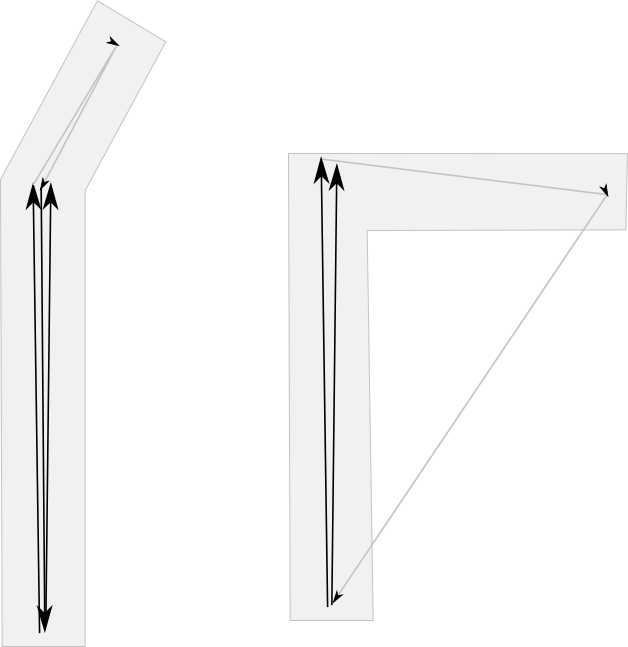
\includegraphics[width=\linewidth]{figures/local_constraints/local_constraints.png}
\caption{Motivation for local constraints. Grey regions represent
  areas where there is evidence for edges.}
\label{fig-local-constraints}
\end{figure}

We use the output of our local interpretation procedure to modify
global inference in two ways:

\begin{itemize}
\item A line segment that goes over an edge pixel with the wrong
  orientation is assigned either $0$ cost (corresponding to the
  assumption that it will be used once in the parse with the correct
  orientation, and once with the reverse orientation) or the negative
  of its normal cost (corresponding to the assumption that it will be
  used twice in the parse with the correct orientation, and once with
  the reverse orientation). The first part of Figure
  \ref{fig-local-constraints} depicts a problematic parse that will be
  penalized appropriately by this heuristic.
\item A line segment is disallowed if too high a fraction of its
  pixels are classified as interior, or if too high a fraction are
  classified as exterior. This is meant to eliminate short-circuiting,
  in which the optimization procedure double-counts an edge by taking
  a round-about way from its head to its tail. Unless the curve
  encompasses the whole object, this test generally prevents
  short-circuiting. The second part of Figure
  \ref{fig-local-constraints} shows an example of short-circuiting.
\end{itemize}

\section{Experimental Results}

\begin{figure*}
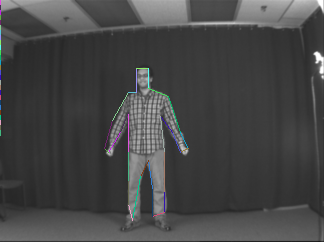
\includegraphics[width=0.48 \linewidth]{output/2.detection/local_inference/out.s1.0010.d/thefinalparse.png}
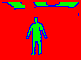
\includegraphics[width=0.48 \linewidth]{output/2.detection/local_inference/out.s1.0010.d/local.x5.interior.png}
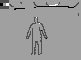
\includegraphics[width=0.24 \linewidth]{output/2.detection/local_inference/out.s1.0010.d/local.x5.orientations.0.png}
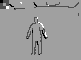
\includegraphics[width=0.24 \linewidth]{output/2.detection/local_inference/out.s1.0010.d/local.x5.orientations.1.png}
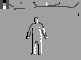
\includegraphics[width=0.24 \linewidth]{output/2.detection/local_inference/out.s1.0010.d/local.x5.orientations.2.png}
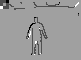
\includegraphics[width=0.24 \linewidth]{output/2.detection/local_inference/out.s1.0010.d/local.x5.orientations.3.png}

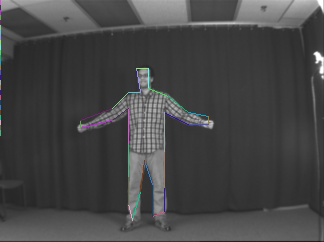
\includegraphics[width=0.48 \linewidth]{output/2.detection/local_inference/out.s1.0020.d/thefinalparse.png}
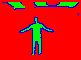
\includegraphics[width=0.48 \linewidth]{output/2.detection/local_inference/out.s1.0020.d/local.x5.interior.png}
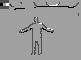
\includegraphics[width=0.24 \linewidth]{output/2.detection/local_inference/out.s1.0020.d/local.x5.orientations.0.png}
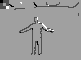
\includegraphics[width=0.24 \linewidth]{output/2.detection/local_inference/out.s1.0020.d/local.x5.orientations.1.png}
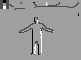
\includegraphics[width=0.24 \linewidth]{output/2.detection/local_inference/out.s1.0020.d/local.x5.orientations.2.png}
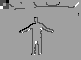
\includegraphics[width=0.24 \linewidth]{output/2.detection/local_inference/out.s1.0020.d/local.x5.orientations.3.png}

\end{figure*}
\begin{figure*}

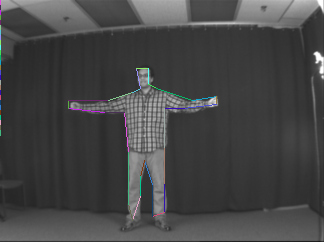
\includegraphics[width=0.48 \linewidth]{output/2.detection/local_inference/out.s1.0030.d/thefinalparse.png}
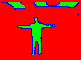
\includegraphics[width=0.48 \linewidth]{output/2.detection/local_inference/out.s1.0030.d/local.x5.interior.png}
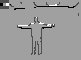
\includegraphics[width=0.24 \linewidth]{output/2.detection/local_inference/out.s1.0030.d/local.x5.orientations.0.png}
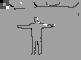
\includegraphics[width=0.24 \linewidth]{output/2.detection/local_inference/out.s1.0030.d/local.x5.orientations.1.png}
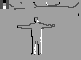
\includegraphics[width=0.24 \linewidth]{output/2.detection/local_inference/out.s1.0030.d/local.x5.orientations.2.png}
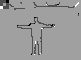
\includegraphics[width=0.24 \linewidth]{output/2.detection/local_inference/out.s1.0030.d/local.x5.orientations.3.png}

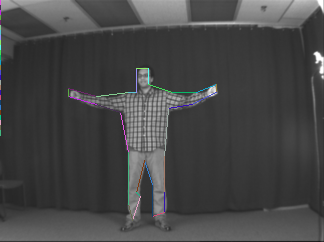
\includegraphics[width=0.48 \linewidth]{output/2.detection/local_inference/out.s1.0040.d/thefinalparse.png}
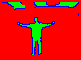
\includegraphics[width=0.48 \linewidth]{output/2.detection/local_inference/out.s1.0040.d/local.x5.interior.png}
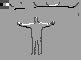
\includegraphics[width=0.24 \linewidth]{output/2.detection/local_inference/out.s1.0040.d/local.x5.orientations.0.png}
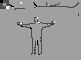
\includegraphics[width=0.24 \linewidth]{output/2.detection/local_inference/out.s1.0040.d/local.x5.orientations.1.png}
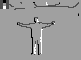
\includegraphics[width=0.24 \linewidth]{output/2.detection/local_inference/out.s1.0040.d/local.x5.orientations.2.png}
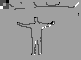
\includegraphics[width=0.24 \linewidth]{output/2.detection/local_inference/out.s1.0040.d/local.x5.orientations.3.png}

\end{figure*}
\begin{figure*}

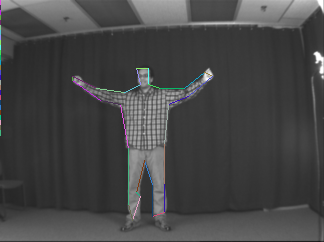
\includegraphics[width=0.48 \linewidth]{output/2.detection/local_inference/out.s1.0050.d/thefinalparse.png}
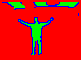
\includegraphics[width=0.48 \linewidth]{output/2.detection/local_inference/out.s1.0050.d/local.x5.interior.png}
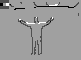
\includegraphics[width=0.24 \linewidth]{output/2.detection/local_inference/out.s1.0050.d/local.x5.orientations.0.png}
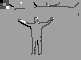
\includegraphics[width=0.24 \linewidth]{output/2.detection/local_inference/out.s1.0050.d/local.x5.orientations.1.png}
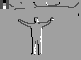
\includegraphics[width=0.24 \linewidth]{output/2.detection/local_inference/out.s1.0050.d/local.x5.orientations.2.png}
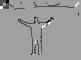
\includegraphics[width=0.24 \linewidth]{output/2.detection/local_inference/out.s1.0050.d/local.x5.orientations.3.png}

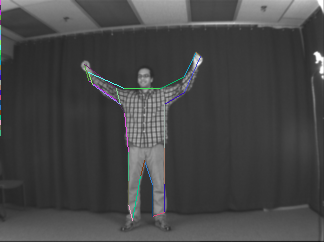
\includegraphics[width=0.48 \linewidth]{output/2.detection/local_inference/out.s1.0060.d/thefinalparse.png}
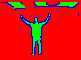
\includegraphics[width=0.48 \linewidth]{output/2.detection/local_inference/out.s1.0060.d/local.x5.interior.png}
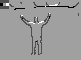
\includegraphics[width=0.24 \linewidth]{output/2.detection/local_inference/out.s1.0060.d/local.x5.orientations.0.png}
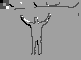
\includegraphics[width=0.24 \linewidth]{output/2.detection/local_inference/out.s1.0060.d/local.x5.orientations.1.png}

\includegraphics[width=0.24 \linewidth]{output/2.detection/local_inference/out.s1.0060.d/local.x5.orientations.2.png}

\includegraphics[width=0.24 \linewidth]{output/2.detection/local_inference/out.s1.0060.d/local.x5.orientations.3.png}

\end{figure*}
\begin{figure*}

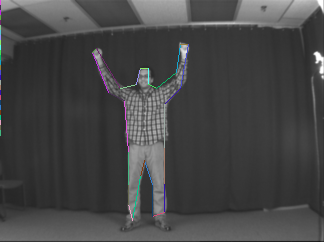
\includegraphics[width=0.48 \linewidth]{output/2.detection/local_inference/out.s1.0070.d/thefinalparse.png}
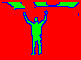
\includegraphics[width=0.48 \linewidth]{output/2.detection/local_inference/out.s1.0070.d/local.x5.interior.png}
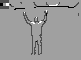
\includegraphics[width=0.24 \linewidth]{output/2.detection/local_inference/out.s1.0070.d/local.x5.orientations.0.png}
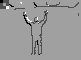
\includegraphics[width=0.24 \linewidth]{output/2.detection/local_inference/out.s1.0070.d/local.x5.orientations.1.png}

\includegraphics[width=0.24 \linewidth]{output/2.detection/local_inference/out.s1.0070.d/local.x5.orientations.2.png}
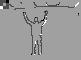
\includegraphics[width=0.24 \linewidth]{output/2.detection/local_inference/out.s1.0070.d/local.x5.orientations.3.png}

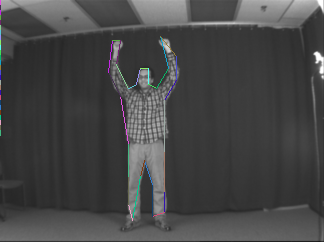
\includegraphics[width=0.48 \linewidth]{output/2.detection/local_inference/out.s1.0080.d/thefinalparse.png}
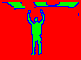
\includegraphics[width=0.48 \linewidth]{output/2.detection/local_inference/out.s1.0080.d/local.x5.interior.png}
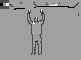
\includegraphics[width=0.24 \linewidth]{output/2.detection/local_inference/out.s1.0080.d/local.x5.orientations.0.png}
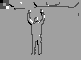
\includegraphics[width=0.24 \linewidth]{output/2.detection/local_inference/out.s1.0080.d/local.x5.orientations.1.png}

\includegraphics[width=0.24 \linewidth]{output/2.detection/local_inference/out.s1.0080.d/local.x5.orientations.2.png}
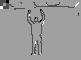
\includegraphics[width=0.24 \linewidth]{output/2.detection/local_inference/out.s1.0080.d/local.x5.orientations.3.png}

\end{figure*}
\begin{figure*}

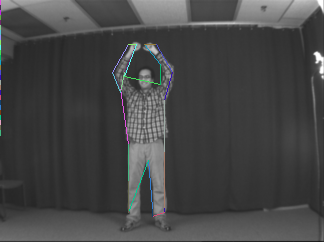
\includegraphics[width=0.48 \linewidth]{output/2.detection/local_inference/out.s1.0090.d/thefinalparse.png}
\includegraphics[width=0.48 \linewidth]{output/2.detection/local_inference/out.s1.0090.d/local.x5.interior.png}
\includegraphics[width=0.24 \linewidth]{output/2.detection/local_inference/out.s1.0090.d/local.x5.orientations.0.png}
\includegraphics[width=0.24 \linewidth]{output/2.detection/local_inference/out.s1.0090.d/local.x5.orientations.1.png}
\includegraphics[width=0.24 \linewidth]{output/2.detection/local_inference/out.s1.0090.d/local.x5.orientations.2.png}
\includegraphics[width=0.24 \linewidth]{output/2.detection/local_inference/out.s1.0090.d/local.x5.orientations.3.png}

\includegraphics[width=0.48 \linewidth]{output/2.detection/local_inference/out.s1.0100.d/thefinalparse.png}
\includegraphics[width=0.48 \linewidth]{output/2.detection/local_inference/out.s1.0100.d/local.x5.interior.png}
\includegraphics[width=0.24 \linewidth]{output/2.detection/local_inference/out.s1.0100.d/local.x5.orientations.0.png}
\includegraphics[width=0.24 \linewidth]{output/2.detection/local_inference/out.s1.0100.d/local.x5.orientations.1.png}
\includegraphics[width=0.24 \linewidth]{output/2.detection/local_inference/out.s1.0100.d/local.x5.orientations.2.png}
\includegraphics[width=0.24 \linewidth]{output/2.detection/local_inference/out.s1.0100.d/local.x5.orientations.3.png}

% \includegraphics[width=0.3 \linewidth]{output/2.detection/local_inference/out.s1.0030.d/thefinalparse.png}
% \includegraphics[width=0.3 \linewidth]{output/2.detection/local_inference/out.s1.0030.d/local.x5.orientations.png}
% \includegraphics[width=0.3 \linewidth]{output/2.detection/local_inference/out.s1.0030.d/local.x5.interior.png}
% \includegraphics[width=0.3 \linewidth]{output/2.detection/local_inference/out.s1.0040.d/thefinalparse.png}
% \includegraphics[width=0.3 \linewidth]{output/2.detection/local_inference/out.s1.0040.d/local.x5.orientations.png}
% \includegraphics[width=0.3 \linewidth]{output/2.detection/local_inference/out.s1.0040.d/local.x5.interior.png}
% \includegraphics[width=0.3 \linewidth]{output/2.detection/local_inference/out.s1.0050.d/thefinalparse.png}
% \includegraphics[width=0.3 \linewidth]{output/2.detection/local_inference/out.s1.0050.d/local.x5.orientations.png}
% \includegraphics[width=0.3 \linewidth]{output/2.detection/local_inference/out.s1.0050.d/local.x5.interior.png}
% \includegraphics[width=0.3 \linewidth]{output/2.detection/local_inference/out.s1.0060.d/thefinalparse.png}
% \includegraphics[width=0.3 \linewidth]{output/2.detection/local_inference/out.s1.0060.d/local.x5.orientations.png}
% \includegraphics[width=0.3 \linewidth]{output/2.detection/local_inference/out.s1.0060.d/local.x5.interior.png}
% \includegraphics[width=0.3 \linewidth]{output/2.detection/local_inference/out.s1.0070.d/thefinalparse.png}
% \includegraphics[width=0.3 \linewidth]{output/2.detection/local_inference/out.s1.0070.d/local.x5.orientations.png}
% \includegraphics[width=0.3 \linewidth]{output/2.detection/local_inference/out.s1.0070.d/local.x5.interior.png}
\end{figure*}
% \begin{figure*}
% \includegraphics[width=0.3 \linewidth]{output/2.detection/local_inference/out.s1.0080.d/thefinalparse.png}
% \includegraphics[width=0.3 \linewidth]{output/2.detection/local_inference/out.8.d/local.x5.orientations.png}
% \includegraphics[width=0.3 \linewidth]{output/2.detection/local_inference/out.8.d/local.x5.interior.png}
% \includegraphics[width=0.3 \linewidth]{output/2.detection/local_inference/out.9.d/thefinalparse.png}
% \includegraphics[width=0.3 \linewidth]{output/2.detection/local_inference/out.9.d/local.x5.orientations.png}
% \includegraphics[width=0.3 \linewidth]{output/2.detection/local_inference/out.9.d/local.x5.interior.png}
% \includegraphics[width=0.3 \linewidth]{output/2.detection/local_inference/out.10.d/thefinalparse.png}
% \includegraphics[width=0.3 \linewidth]{output/2.detection/local_inference/out.10.d/local.x5.orientations.png}
% \includegraphics[width=0.3 \linewidth]{output/2.detection/local_inference/out.10.d/local.x5.interior.png}
% \includegraphics[width=0.3 \linewidth]{output/2.detection/local_inference/out.11.d/thefinalparse.png}
% \includegraphics[width=0.3 \linewidth]{output/2.detection/local_inference/out.11.d/local.x5.orientations.png}
% \includegraphics[width=0.3 \linewidth]{output/2.detection/local_inference/out.11.d/local.x5.interior.png}
% \includegraphics[width=0.3 \linewidth]{output/2.detection/local_inference/out.12.d/thefinalparse.png}
% \includegraphics[width=0.3 \linewidth]{output/2.detection/local_inference/out.12.d/local.x5.orientations.png}
% \includegraphics[width=0.3 \linewidth]{output/2.detection/local_inference/out.12.d/local.x5.interior.png}
% \includegraphics[width=0.3 \linewidth]{output/2.detection/local_inference/out.13.d/thefinalparse.png}
% \includegraphics[width=0.3 \linewidth]{output/2.detection/local_inference/out.13.d/local.x5.orientations.png}
% \includegraphics[width=0.3 \linewidth]{output/2.detection/local_inference/out.13.d/local.x5.interior.png}
% \end{figure*}
% \begin{figure*}
% \includegraphics[width=0.3 \linewidth]{output/2.detection/local_inference/out.14.d/thefinalparse.png}
% \includegraphics[width=0.3 \linewidth]{output/2.detection/local_inference/out.14.d/local.x5.orientations.png}
% \includegraphics[width=0.3 \linewidth]{output/2.detection/local_inference/out.14.d/local.x5.interior.png}
% \includegraphics[width=0.3 \linewidth]{output/2.detection/local_inference/out.15.d/thefinalparse.png}
% \includegraphics[width=0.3 \linewidth]{output/2.detection/local_inference/out.15.d/local.x5.orientations.png}
% \includegraphics[width=0.3 \linewidth]{output/2.detection/local_inference/out.15.d/local.x5.interior.png}
% \end{figure*}
